\chapter{Material adicional}
\label{chap:adicional}

\lettrine{E}{xemplo} de capítulo con formato de apéndice, onde se pode
incluír material adicional que non teña cabida no corpo principal do
documento, suxeito á limitación de 80 páxinas establecida no
regulamento de TFGs.

\Blindtext


\chapter{Descrición dos casos de uso principais}
\label{chapapd:descricion-casos-principais}

Nesta sección descríbense con maior detalle os casos de uso máis representativos do funcionamento do sistema. Seleccionáronse aqueles que recollen os principais fluxos da aplicación e as interaccións máis relevantes entre o paciente, o supervisor, a API e os servizos externos.

\subsubsection{CU-02: Vincular paciente e supervisor}

\begin{description}
    \item[Actores:] Paciente e supervisor.

    \item[Precondicións:] Ambos os dispositivos teñen a aplicación iniciada, dispoñen de conexión á rede e completaron a selección do seu rol. O supervisor dispón de permisos para utilizar a cámara.

    \item[Disparador:] O paciente selecciona a opción de xerar un código QR para vincular un supervisor.

    \item[Fluxo principal:] \hfill
    \begin{enumerate}
        \item A aplicación informa de que a persoa vinculada poderá consultar a información compartida, recibir avisos e dixitalizar novas follas no nome do paciente.
        \item O paciente solicita a xeración do código QR, aceptando os permisos asociados á vinculación.
        \item A aplicación do paciente xera un código QR cos identificadores e os datos de seguridade necesarios.
        \item O supervisor abre a opción de lectura, escanea o código e o sistema comproba a súa validez.
        \item Os dispositivos intercambian as credenciais necesarias para establecer unha canle de comunicación segura.
        \item O paciente pasa a figurar como vinculado no dispositivo do supervisor.
        \item A vinculación actívase e os dispositivos poden intercambiar o estado do tratamento de forma protexida.
        \item O supervisor pode consultar os datos sincronizados e dixitalizar novas follas no nome do paciente.
    \end{enumerate}

    \item[Fluxos alternativos:] Se o código QR ten un formato incorrecto ou xa foi empregado, a aplicación rexeita a vinculación e solicita xerar outro código. En caso de fallo de conexión ou se as credenciais de seguridade non se poden verificar, a operación cancélase indicando o motivo. O paciente pode omitir este proceso e empregar a aplicación de maneira autónoma.

    \item[Postcondicións:] Establécese unha relación de confianza entre os dispositivos. A vinculación permite ao supervisor consultar a información compartida, recibir avisos e dixitalizar novas follas no nome do paciente. Estes permisos poden retirarse mediante a revogación da vinculación desde os axustes da aplicación.
\end{description}

O intercambio de información necesario para establecer a vinculación entre os dous dispositivos represéntase no diagrama de secuencia da Figura~\ref{fig:cu02-vinculacion}.

\begin{figure}
    \centering
    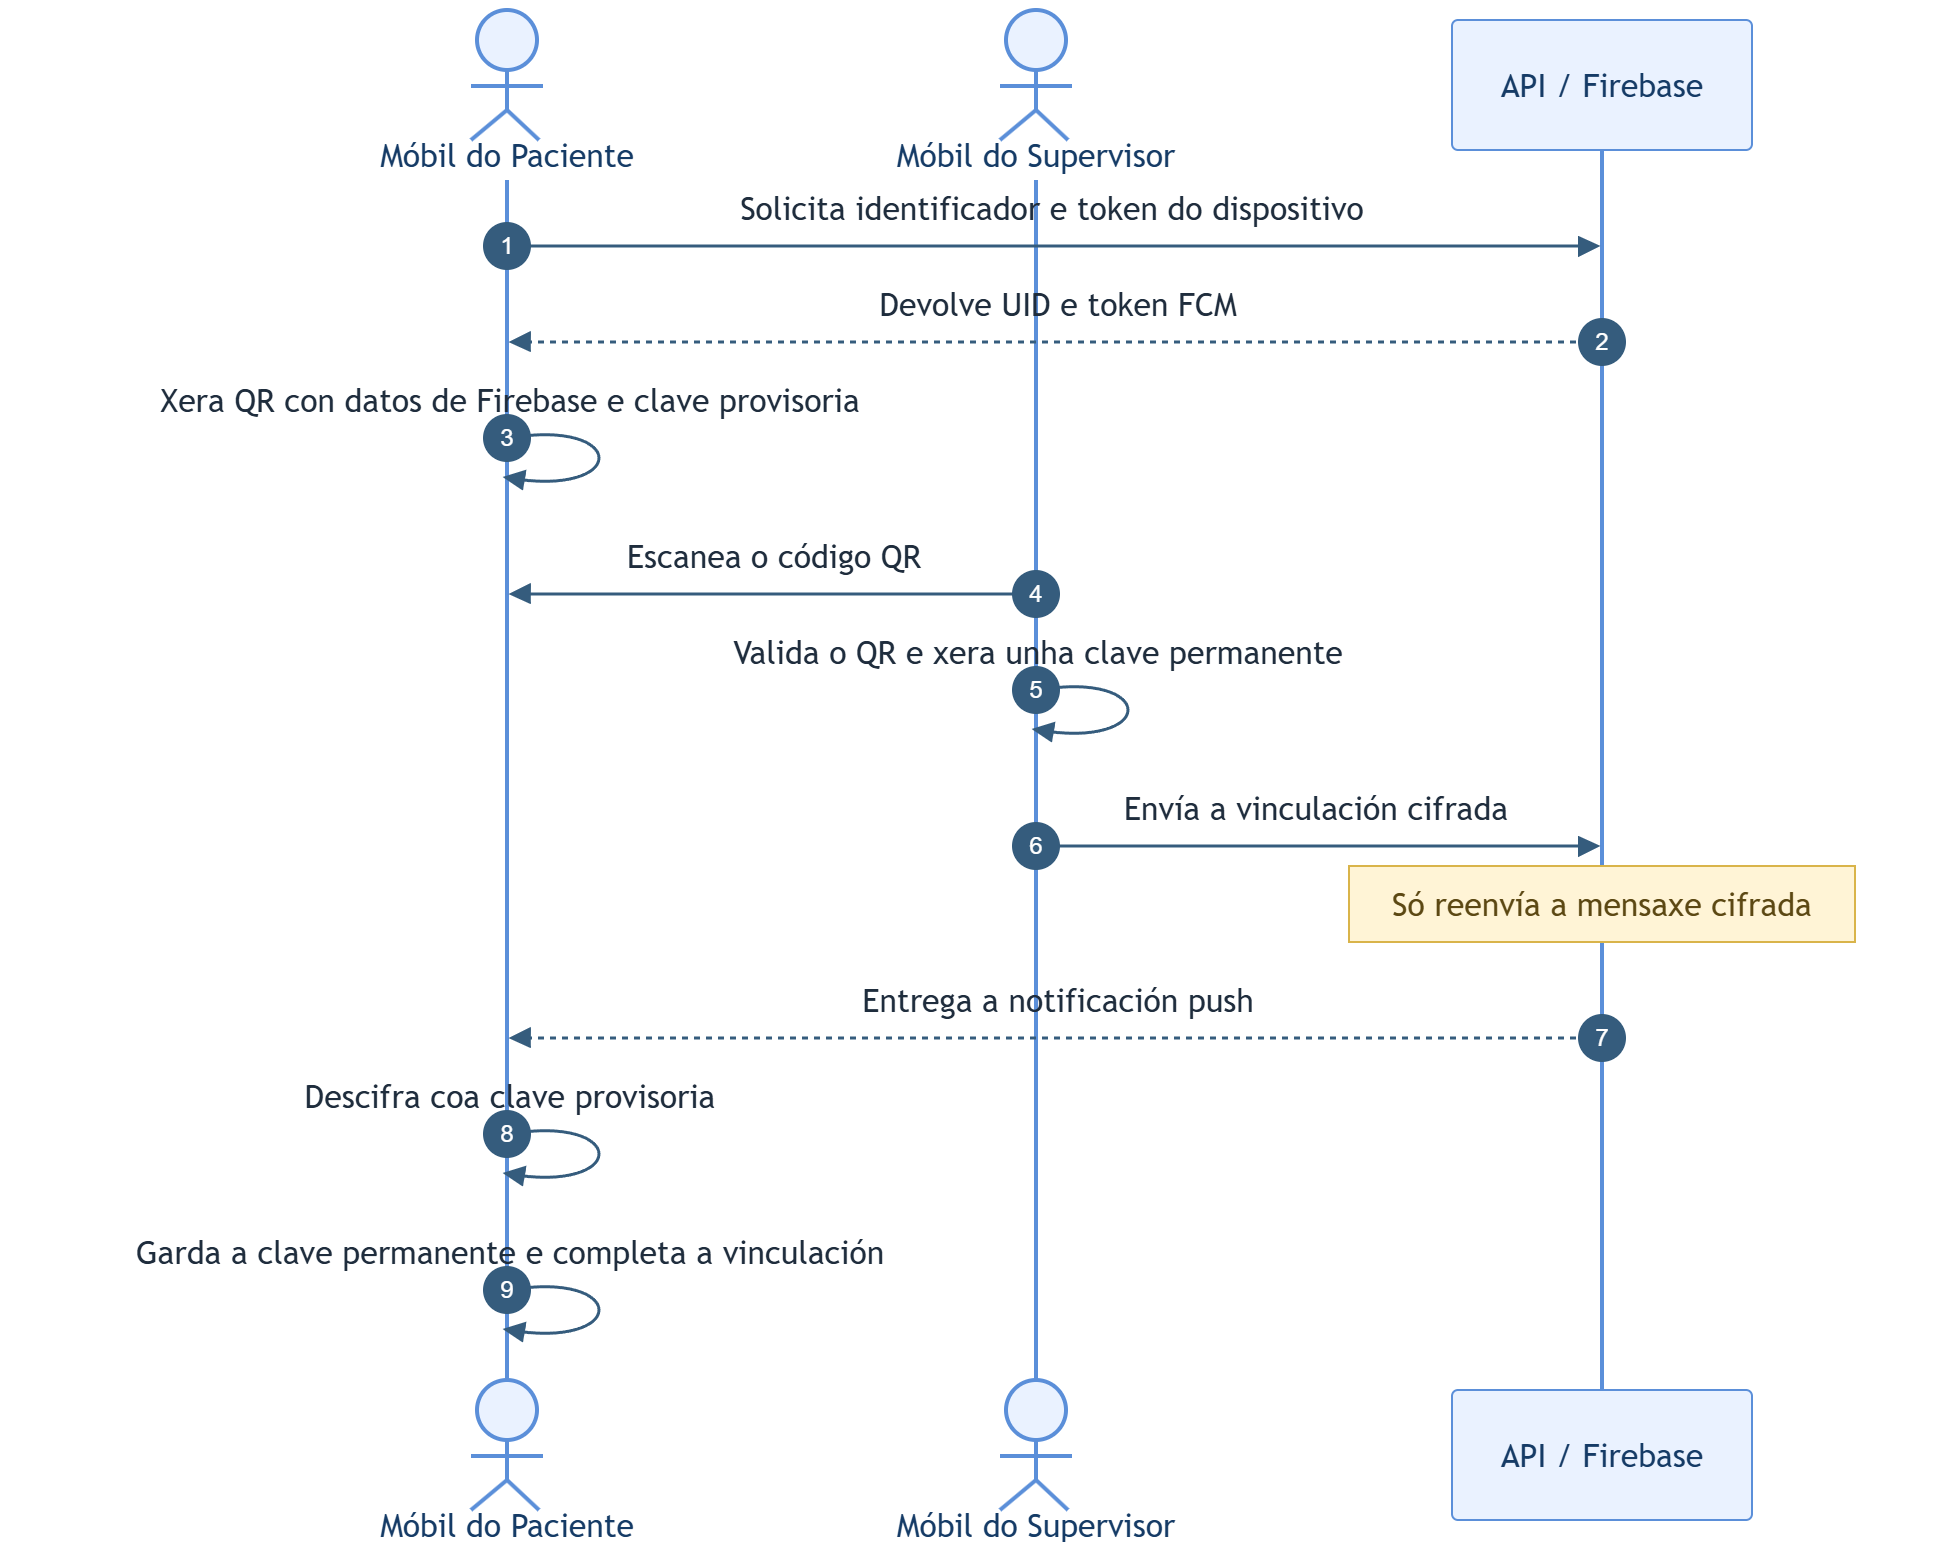
\includegraphics[width=1\linewidth]{imaxes/04-Analise/CU02-Vinculacion.png}
    \caption{Diagrama de secuencia do proceso de vinculación entre o paciente e o supervisor (CU-02).}
    \label{fig:cu02-vinculacion}
\end{figure}
\FloatBarrier

\subsubsection{CU-04: Procesar unha folla de tratamento}

\begin{description}
    \item[Actor principal:] Paciente ou supervisor vinculado.

    \item[Precondicións:] A aplicación está iniciada, existe conexión á rede e o actor dispón dunha folla de tratamento lexible. Se a acción a realiza un supervisor, este debe manter unha vinculación activa co paciente e telo seleccionado previamente.

    \item[Disparador:] O usuario preme a opción de engadir ou actualizar unha folla de tratamento.

    \item[Fluxo principal:] \hfill
    \begin{enumerate}
        \item O usuario selecciona a orixe do documento: cámara, galería ou ficheiro PDF.
        \item A aplicación comproba que o formato e o tamaño sexan compatibles.
        \item O ficheiro envíase á API mediante unha petición HTTPS.
        \item A API preprocesa a imaxe, extrae os datos estruturados e aplica as regras de validación.
        \item Se a API procesa correctamente o documento, a aplicación recibe os datos extraídos e gárdaos localmente.
        \item A nova pauta móstrase na interface principal.
        \item Se existen outros dispositivos vinculados, a actualización empaquétase de forma segura e sincronízase automaticamente con eles.
    \end{enumerate}

    \item[Fluxos alternativos:] Se o documento non é lexible, a API rexeita o formato ou faltan datos obrigatorios, o proceso interrómpese. A aplicación mantén intacta a pauta anterior, mostra unha mensaxe de erro descritiva e solicita repetir a captura. Se a extracción se completa pero falla a sincronización, a pauta permanece gardada no dispositivo local e infórmase do erro de rede.

    \item[Postcondicións:] A nova pauta consolídase no dispositivo que realizou a operación e sincronízase de forma segura cos dispositivos vinculados. O documento orixinal descártase tras a súa análise e non se almacena de forma persistente no servidor.
\end{description}

As diferentes etapas do procesamento e o comportamento do sistema ante un resultado correcto ou un erro represéntanse no diagrama de actividade da Figura~\ref{fig:cu04-procesar-folla}.

\begin{figure}[H]
    \centering
    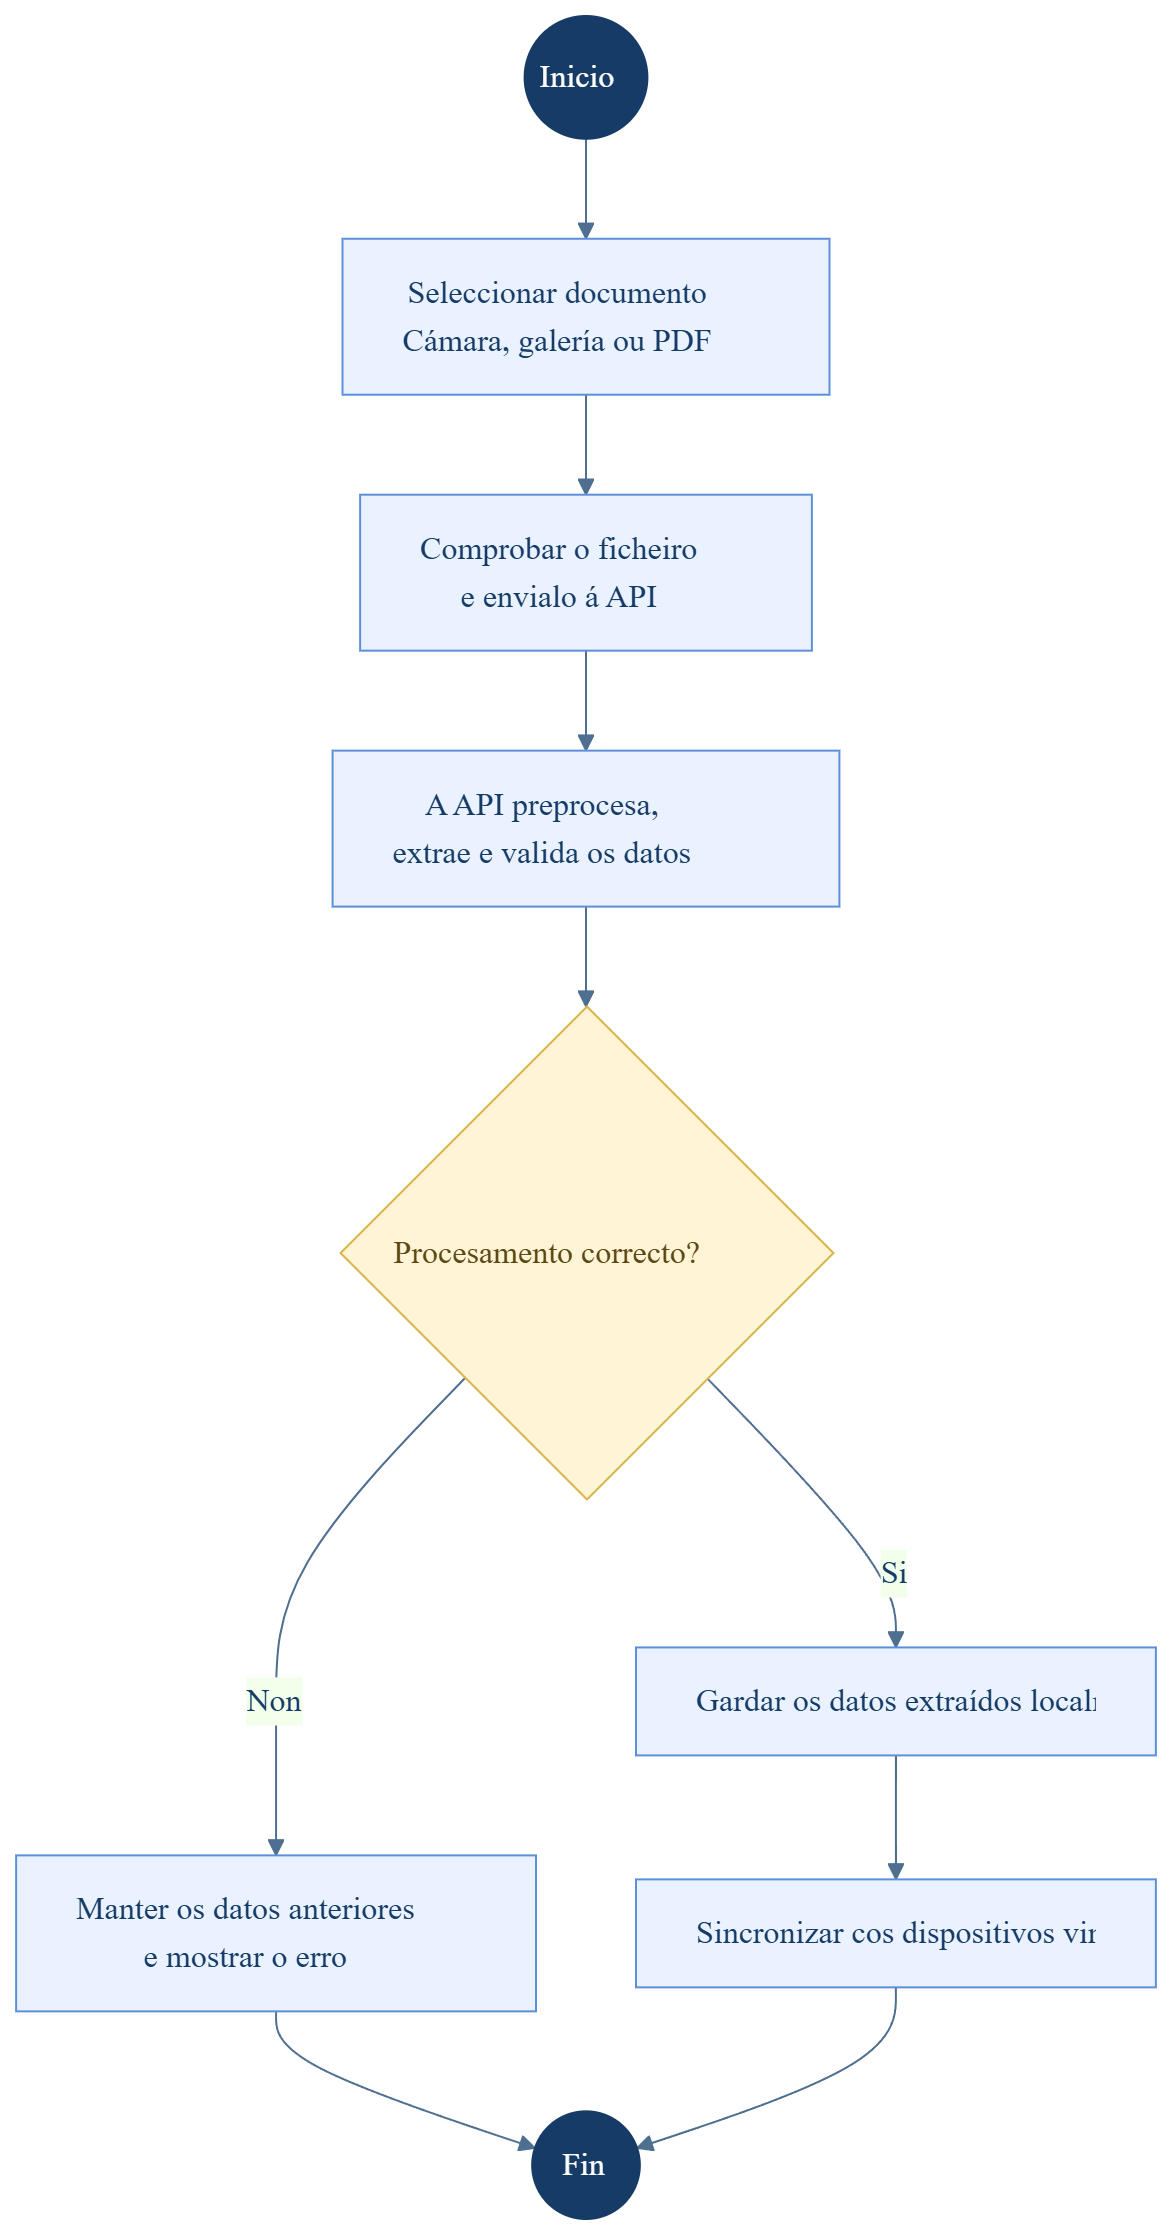
\includegraphics[width=0.6\linewidth]{imaxes/04-Analise/CU04-Procesar-Folla.png}
    \caption{Diagrama de actividade do procesamento dunha folla de tratamento (CU-04).}
    \label{fig:cu04-procesar-folla}
\end{figure}
\FloatBarrier

\subsubsection{CU-06: Confirmar unha toma}

\begin{description}
    \item[Actor principal:] Paciente.

    \item[Precondicións:] O sistema conta cunha pauta activa que inclúe unha dose prescrita para o día en curso.

    \item[Disparador:] O paciente activa o control de confirmación da toma diaria na interface.

    \item[Fluxo principal:] \hfill
    \begin{enumerate}
        \item A aplicación identifica a dose asignada para a xornada actual.
        \item Rexistra a confirmación xunto coa data e a hora exactas na base de datos local.
        \item Avalía a puntualidade da toma en comparación coa hora habitual configurada nas preferencias.
        \item Actualiza a pantalla de inicio, o calendario e as métricas de adherencia.
        \item Se existen supervisores vinculados, notifícase o evento aos seus dispositivos de forma segura.
    \end{enumerate}

    \item[Fluxos alternativos:] A interface non permite confirmar unha toma cando a pauta indica que ese día non debe tomarse medicación ou corresponde unicamente a un control médico. En ausencia de conexión, a confirmación permanece rexistrada localmente, pero a comunicación cos supervisores non pode completarse ata recuperar a conectividade.

    \item[Postcondicións:] A toma pasa ao estado de confirmada e incorpórase ao historial local de tomas. Os supervisores que reciban correctamente a actualización poden consultar o novo estado.
\end{description}

Os posibles estados asociados á toma diaria e as transicións producidas pola confirmación represéntanse na Figura~\ref{fig:cu06-confirmar-toma}.

\begin{figure}[H]
    \centering
    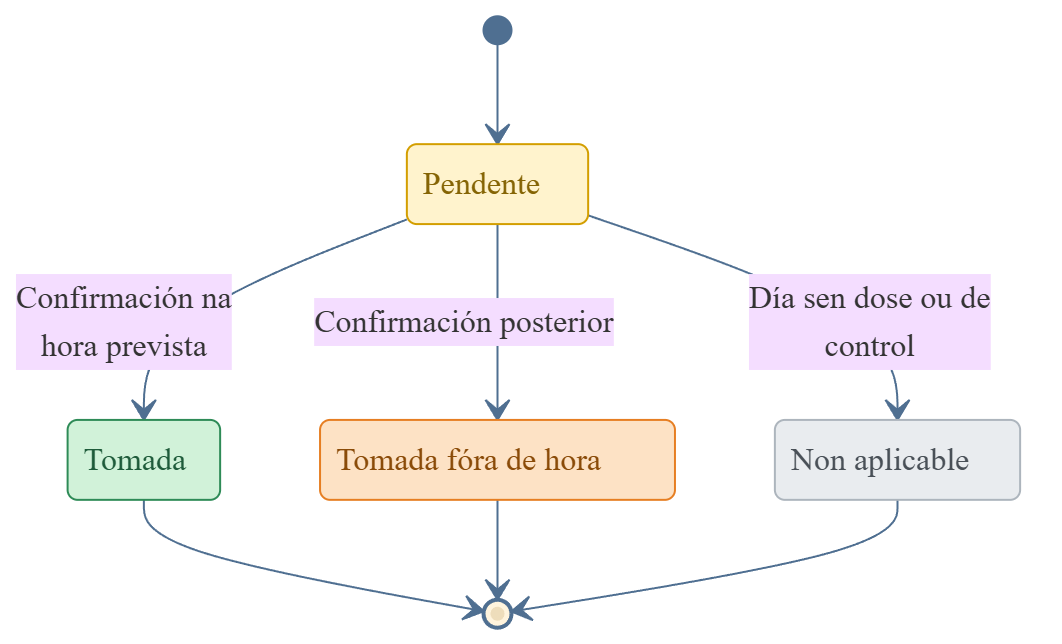
\includegraphics[width=0.6\linewidth]{imaxes/04-Analise/CU06-Confirmar-Toma.png}
    \caption{Diagrama de estados asociado á confirmación dunha toma diaria (CU-06).}
    \label{fig:cu06-confirmar-toma}
\end{figure}
\FloatBarrier

\subsubsection{CU-10: Supervisar un paciente}

\begin{description}
    \item[Actor principal:] Supervisor.

    \item[Precondicións:] O supervisor mantén unha vinculación activa con polo menos un paciente que xa compartiu información do seu tratamento.

    \item[Disparador:] O supervisor selecciona un perfil de paciente na pantalla principal.

    \item[Fluxo principal:] \hfill
    \begin{enumerate}
        \item A aplicación carga o panel de estado do paciente seleccionado.
        \item O supervisor visualiza a dose do día, o estado da toma e a data da seguinte visita médica.
        \item O supervisor pode consultar o calendario e as gráficas de evolución dispoñibles.
        \item O supervisor pode iniciar a captura dunha nova folla para actualizar a pauta do paciente seleccionado.
        \item Se o documento se procesa correctamente, a nova pauta envíase de forma segura ao dispositivo do paciente.
    \end{enumerate}

    \item[Fluxos alternativos:] Se o paciente aínda non dixitalizou ningunha folla, móstrase unha mensaxe indicando que non hai información dispoñible. Se a vinculación foi revogada, o sistema bloquea o acceso ao perfil, impide dixitalizar novas follas no seu nome e deixa de aceptar actualizacións asociadas á relación eliminada.

    \item[Postcondicións:] A consulta non modifica o estado do tratamento. Se o supervisor procesa unha nova folla, a pauta actualízase e sincronízase co paciente vinculado.
\end{description}

\subsubsection{CU-11: Sincronizar cambios e recibir avisos}

\begin{description}
    \item[Actor principal:] Paciente ou supervisor.

    \item[Precondicións:] Existe unha vinculación activa e comprobada entre os dispositivos.

    \item[Disparador:] Prodúcese un cambio que debe ser comunicado, como a confirmación dunha toma, a actualización dunha pauta, unha modificación da configuración ou a revogación dunha vinculación.

    \item[Fluxo principal:] \hfill
    \begin{enumerate}
        \item O dispositivo de orixe empaqueta a actualización e cífraa, garantindo a súa privacidade.
        \item A API recibe a petición de envío e encamíñaa ao destinatario correspondente sen acceder ao contido da mensaxe.
        \item O dispositivo destinatario recibe a notificación e verifica a autenticidade e a integridade da mensaxe.
        \item Se a comprobación é correcta, descifra a información, aplícaa e actualiza a interface.
    \end{enumerate}

    \item[Fluxos alternativos:] Se a orixe é descoñecida, a mensaxe foi alterada durante o tránsito ou non cumpre os controis de seguridade, o dispositivo descártaa sen modificar os datos locais. Se non hai conexión á rede, o envío non pode completarse, pero consérvanse os datos gardados no dispositivo de orixe para permitir unha sincronización posterior.

    \item[Postcondicións:] O dispositivo destinatario incorpora unha actualización procedente dunha vinculación válida. A API e o servizo de mensaxería interveñen unicamente como intermediarios e non acceden á información clínica en claro.
\end{description}

O proceso de envío dunha actualización cifrada e o papel da API e de Firebase como intermediarios represéntanse no diagrama de secuencia da Figura~\ref{fig:cu11-sincronizacion-avisos}.

\begin{figure}
    \centering
    \includegraphics[width=1\linewidth]{imaxes/04-Analise/cu11-sincronizacion-avisos.png}
    \caption{Diagrama de secuencia da sincronización segura de cambios e avisos entre dispositivos (CU-11).}
    \label{fig:cu11-sincronizacion-avisos}
\end{figure}
\FloatBarrier
